\documentclass{ctexart}

% \usepackage{AcademicReportCn}

% enable Chinese
% \usepackage[UTF8]{ctex}

% setting for levels
% \usepackage{hyperref}
% \setcounter{secnumdepth}{2}
% \setcounter{tocdepth}{2}
% \hypersetup{
%     bookmarksopenlevel = 3,
%     citecolor = red,
% 	colorlinks		=	true,
% 	bookmarks		=	true,
% 	bookmarksopen	=	true,
%     % bookmarksdepth  =   2,
% 	pdfstartview	=	Fit,
% 	pdftitle		=	{画图建议指南},
% 	pdfauthor		=	{钟家鑫},
% }

% biber is required to compile: xelatex -> biber -> xelatex*2
% \usepackage[
%     giveninits=true, 
%     maxbibnames=99,
%     % style=numeric,
%     sorting=none,
%     doi = false,
%     url = false,
%     isbn = false,
%     style=ieee, citestyle=numeric-comp,
%     ]{biblatex}
% \addbibresource{biblatex.bib}

% open book mark at arbitrary level
% \usepackage[open, numbered]{bookmark}
% opt: numbered --- show numbers in the bookmark

\usepackage{graphicx}
% \usepackage{subcaption}

% see https://tex.stackexchange.com/questions/226481/appendix-section-title
% \usepackage[title]{appendix}


\title{\textbf{画图建议指南}}
\author{钟家鑫}
\date{\today}

% \usepackage{mlmodern}
% reduce space between enumerated items
% \usepackage{enumitem}
% \setlist{nolistsep}


\begin{document}
\maketitle
% enable Page 1 of xx at the first page
% \thispagestyle{firststyle}

\section{简介}
本文档总结论文画图的一些建议。

\section{二维图}
图~\ref{fig:2d_fig}~由附件的demo.m文件生成。
主要注意事项包括:
\begin{itemize}
    \item 字体尽可能大。
    \item 若横纵坐标表示实际物理的长度,则比例应与物理的长度比例相同。如图~\ref{fig:2d_fig}~中长宽比例就当为$8\,\mathrm{m} : 4\, \mathrm{m} = 2:1$。
    \item 图中所有文字采用字体 Times New Roman,xlabel 和 ylabel 等采用 LaTeX 为 Interpreter。
    \item 输出的图为矢量图,如 *.pdf。
    \item 选择更现代化的 colormap,图~\ref{fig:2d_fig}~选择的是vik \cite{Crameri2020MisuseColourScience}。
\end{itemize}

\begin{figure}[!htb]
    \centering
    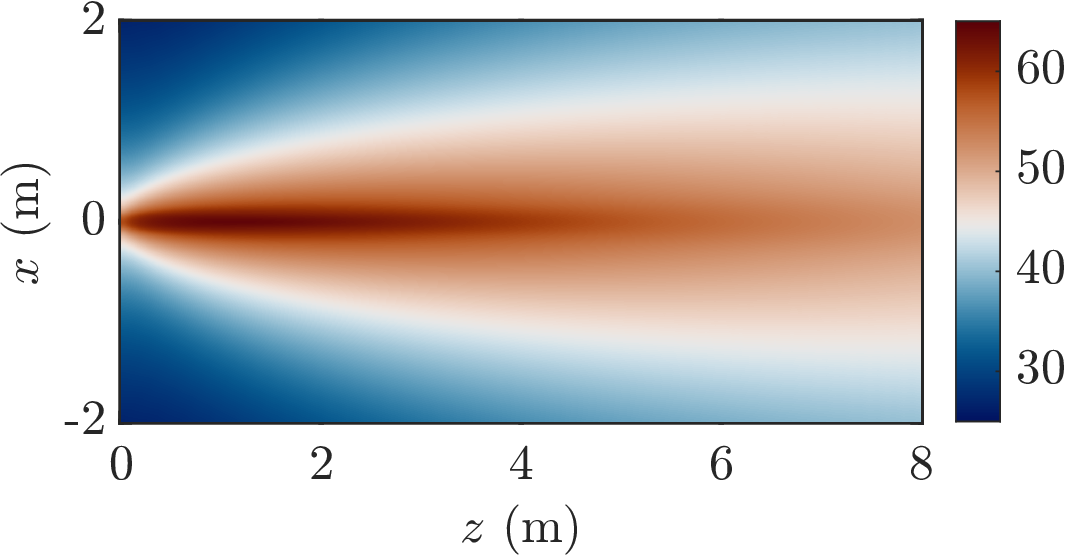
\includegraphics[width = 0.6\textwidth]{fig}
    \caption{二维音频声场声压级分布图}
    \label{fig:2d_fig}
\end{figure}



% \addcontentsline{toc}{section}{参考文献}
% https://tex.stackexchange.com/questions/261443/changing-bibliography-title-with-biblatex-within-the-document
% \printbibliography[title=参考文献]
\bibliographystyle{unsrt}
\bibliography{bibtex}

\end{document}


